\chapter{Analisis}
\label{chap:analisis}

Pada bab ini akan dibahas mengenai analisis Twitter API, OAuth, KIRI API, Twitter4J, Spesifikasi kebutuhan fungsional, Diagram \textit{Use Case}, dan \textit{Diagram Class}.

\section{Analisis Data}

Pada sub bab ini, akan dilakukan analisa tentang Twitter API, OAuth, KIRI API, dan Twitter4j. Setelah membaca dan menganalisis maka penulis akan menentukan hal-hal  yang akan digunakan dalam membangun \textit{Twitter bot} untuk mencari jalur transportasi publik.

\subsection{Analisis Twitter API}
Setelah melakukan analisis, perangkat lunak yang akan dibangun menggunakan \textit{Streaming} API karena:
\begin{itemize}
	\item Streaming API adalah \textit{real-time} API, sedangkan \textit{search} API hanya dapat menangkap \textit{tweet} setiap beberapa waktu sekali. Pada perangkat lunak yang akan dibuat skenarionya adalah pengguna akan menanyakan rute transportasi publik dalam bentuk \textit{tweet} yang dikirimkan kepada akun \textit{Twitter bot}, dalam skenario seperti ini dibutuhkan jawaban yang \textit{real-time}.
	\item \textit{Endpoint streaming} menggunakan \textit{public stream}. \textit{Public Stream} mengambil semua data publik, sehingga semua \textit{tweet} bisa ditangkap oleh perangkat lunak. Dalam pembuatan \textit{Twitter Bot} untuk mencari jalur transportasi publik, pengguna akan melakukan \textit{mention tweet} kepada akun \textit{Twitter bot} untuk dapat memperoleh balasan \textit{tweet} yang berisi hasil pencarian jalur transportasi publik. \textit{Public Stream} mempunyai fitur bernama \textit{track}. Fitur \textit{track} berguna untuk menyaring \textit{tweet} berdasarkan \textit{keyword} tertentu. \textit{Keyword} yang akan di-\textit{track} adalah nama akun dari \textit{Twitter bot}, jadi perangkat lunak hanya menerima \textit{tweet} yang di-\textit{mention} kepada akun \textit{Twitter bot} saja. \textit{User stream} mengandung semua data yang berhubungan dengan satu akun tertentu seperti \textit{update status}, \textit{mention}, dan \textit{direct message}. Dalam kasus ini bisa saja menggunakan \textit{user stream} tetapi penggunaannya kurang efisien. Pengambilan \textit{tweet update status} dan \textit{direct message} tidak dibutuhkan dalam pembuatan perangkat lunak \textit{Twitter bot}. \textit{Site stream} merupakan versi \textit{multi-user stream}. Dalam kasus \textit{Twitter bot} untuk mencari jalur transportasi publik ini akun yang digunakan untuk menjadi \textit{Twitter bot} hanya satu akun saja. Jadi penggunaan \textit{site stream} dalam kasus ini kurang efisien.
\end{itemize}

\subsection{Analisis OAuth}
Setelah melakukan analisis, OAuth yang digunakan dalam pembuatan \textit{Twitter bot} untuk mencari jalur transportasi publik adalah \textit{3-legged authorization}. Penggunaan \textit{3-legged authorization} ini digunakan untuk melakukan otentikasi akun \textit{Twitter bot}. Proses otentikasi tidak perlu dilakukan kepada pengguna, karena \textit{Twitter bot} yang dibuat menggunakan otentikasi langsung dari pengembang perangkat lunak. \textit{Application-only authentication} tidak bisa digunakan karena \textit{application-only authentication} tidak dapat melakukan \textit{posting} \textit{tweet} dan tidak dapat melakukan koneksi dengan \textit{streaming endpoint}. Sedangkan dalam kasus \textit{Twitter bot} untuk mencari jalur transportasi publik dibutuhkan otentikasi yang dapat memposting \textit{tweet} dan melakukan koneksi dengan \textit{streaming endpoint}. Penggunaan otentikasi \textit{PIN-based authorization} tidak cocok, karena otentikasi sudah dilakukan langsung dari pengembang perangkat lunak. Maka dari itu tidak diperlukan PIN untuk proses otentikasi.

\subsection{Analisis KIRI API}
KIRI API menyediakan tiga layanan yang dapat digunakan. \textit{Twitter bot} yang akan dibangun membutuhkan dua layanan yang diberikan KIRI API. Layanan tersebut adalah \textit{Routing Web Service} dan \textit{Search Place Web Service}. \textit{Routing Web Service} adalah layanan yang digunakan untuk mendapatkan langkah perjalanan dari lokasi awal menuju lokasi tujuan. Sedangkan \textit{Search Place Web Service} berguna untuk menemukan rute perjalanan berdasarkan \textit{latitute} dan \textit{longitude} koordinat. Layanan \textit{Search Place Web Service} ini membantu mengubah \textit{latitude} dan \textit{longitude} ke-dalam bentuk string.

Untuk setiap permintaan terhadap KIRI API dibutuhkan \textit{API key}. \textit{API key} ini sendiri berguna sebagai \textit{password} untuk mengakses KIRI API. \textit{API key} ini sendiri dapat didapatkan di \url{https://dev.kiri.travel/bukitjarian/}. Dalam pembuatan \textit{Twitter bot} untuk mencari jalur transportasi publik ini, KIRI memberikan \textit{API key} khusus yaitu 889C2C8FBB82C7E6.

Berikut adalah contoh pemanfaatan KIRI API :

\begin{itemize}
	\item \textit{Search Place Web Service}
	
	Format \textit{Search Place Web Service} yang dikirim melalui URL adalah \url{kiri.travel\/handle.php?version=2\&mode=searchplace\&region=cgk\/bdo\/sub\&querystring="string"\&apikey=889C2C8FBB82C7E6}.
	
	Parameter yang dikirimkan adalah :
	
	\begin{enumerate}
		\item version : 2
		
		Version 2 merupakan versi KIRI API yang terbaru. Oleh karena itu, penulis akan menuliskan parameter version dengan nilai 2.
		\item mode : "searchplace"
		
		Mode "searchplace" merupakan mode dari \textit{Search Place Web Service} yang digunakan untuk mencari lokasi.
		\item region : bdo
		
		\textit{Region} berfungsi sebagai parameter untuk memberitahukan kota yang akan menjadi bagian dalam pencarian lokasi. Parameter yang terdapat di region ada tiga yaitu "cgk" untuk Kota Jakarta, "bdo" untuk Kota Bandung, dan "sub" untuk Kota Surabaya.
		\item querystring
		
		Merupakan kata kunci untuk lokasi.
		\item apikey : 889C2C8FBB82C7E6
		
		Merupakan \textit{password} yang digunakan untuk mengakses KIRI API.
	\end{enumerate}
	
	Penulis mencoba mencari lokasi pvj dari kata kata kunci "pvj" yang berada di Kota Bandung. Layanan dikirimkan ke URL \url{kiri.travel/handle.php}. Berikut adalah format layanan yang dituliskan: \url{http://kiri.travel/handle.php?version=2&mode=searchplace&region=bdo&querystring=pvj&apikey=889C2C8FBB82C7E6}
	
	Berikut adalah hasil kembalian dari KIRI API:
	
	\begin{lstlisting} [caption= hasil kembalian dari \textit{Search Place Web Service}]
	{
			"status":"ok",
			"searchresult":[
					{
						"placename":"J.Co Donuts & Coffee",
						"location":"-6.88929,107.59574"
					},
					{
						"placename":"Pepper Lunch Bandung (PVJ)",
						"location":"-6.88923,107.59615"
					},
					{
						"placename":"Domino's Pizza Pvj",
						"location":"-6.90348,107.61709"
					},
					{
						"placename":"Outlet Alleira Batik PVJ Bandung",
						"location":"-6.88875,107.59634"
					},
					{
						"placename":"Burger King Bandung PVJ Mall",
						"location":"-6.88894,107.59342"
					},
					{
						"placename":"Killiney Kopitiam PVJ",
						"location":"-6.88947,107.59654"
					},
					{
						"placename":"Adidas Pvj",
						"location":"-6.88909,107.59614"
					},
					{
						"placename":"Crocs - PVJ",
						"location":"-6.88894,107.59342"
					},
					{
						"placename":"Cross Pvj",
						"location":"-6.88906,107.59619"
					},
					{
						"placename":"Jonas Photo - PVJ",
						"location":"-6.88913,107.59643"
					}
				],
				"attributions":null
	}\end{lstlisting}
	
	\item \textit{Routing Web Service}
	
	Format \textit{Routing Web Service} yang dikirim melalui URL adalah \url{kiri.travel/handle.php?version=2&mode=findroute&locale=en/id&start=lat,lng&finish=lat,lng&presentation=mobile/desktop&apikey=889C2C8FBB82C7E6}.
	
	Parameter yang dikirimkan adalah :
	
	\begin{enumerate}
		\item version : 2
		
		Version 2 merupakan versi KIRI API yang terbaru. Oleh karena itu, penulis akan menuliskan parameter version dengan nilai 2.
		\item mode : "findroute"
		
		Mode "findroute" merupakan mode dari \textit{Routing Web Service} yang digunakan untuk mendapatkan langkah yang harus dilakukan dari lokasi awal menuju lokasi tujuan.
		\item locale : id
		
		\textit{locale} berfungsi sebagai parameter untuk bahasa yang digunakan. Karena target dari perangkat lunak ini adalah orang Indonesia, maka parameter locale menggunakan "id" untuk Bahasa Indonesia, jika ingin menggunakan Bahasa Ingris maka menggunakan parameter "en".
		\item start
		
		Merupakan koordinat awal. Parameter ini berupa latitude dan longitude.
		\item finish
		
		Merupakan koordinat tujuan. Parameter ini berupa latitude dan longitude.
		\item presentation : "desktop"
		
		Parameter \textit{presentation} ini terdapat dua jenis yaitu "mobile" untuk perangkat bergerak dan "desktop" untuk komputer. Perbedaan mobile dan desktop terletak pada \textit{icon} yang diberikan. Jika menggunakan presentation "mobile" maka hasil kembalian akan terdapat \%toicon dan \%fromicom, hasil tersebut tidak dibutuhkan oleh pengguna karena pengguna \textit{Twitter bot} tidak dapat melihat map jalur transportasi publik yang diberikan.
		\item apikey : 889C2C8FBB82C7E6
		
		Merupakan password yang digunakan untuk mengakses KIRI API.
	\end{enumerate}
	
	Penulis mencoba mencari rute perjalanan dari PVJ(Paris van Java) menuju BIP(Bandung Indah Plaza). Layanan dikirimkan ke URL \url{kiri.travel/handle.php}. Berikut adalah format layanan yang dituliskan:
	\url{http://kiri.travel/handle.php?version=2\&mode=findroute\&locale=en\&start=-6.88923,107.59615\&finish=-6.90864,107.61108\&presentation=desktop\&apikey=889C2C8FBB82C7E6}.
	
	Berikut adalah hasil kembalian dari KIRI API:
	
	\begin{lstlisting} [caption= hasil kembalian dari \textit{Routing Web Service}]
	{
			"status":"ok",
			"routingresults":[
			{
				"steps":[
					[
						"walk",
						"walk",
						["-6.88923,107.59615","-6.88958,107.59691"],
						"Walk about 92 meter from your starting point to Jalan Sukajadi.",
						null
					],
					[
						"angkot",
						"kalapakarangsetra",
						["-6.88958,107.59691","-6.89052,107.59696","-6.89146,107.59701",
						"-6.89239,107.59706","-6.89333,107.59711","-6.89333,107.59711",
						"-6.89466,107.59719","-6.89598,107.59727","-6.89598,107.59727",
						"-6.89700,107.59731","-6.89801,107.59735","-6.89903,107.59740",
						"-6.90005,107.59744","-6.90005,107.59744","-6.90113,107.59747",
						"-6.90222,107.59751","-6.90331,107.59754","-6.90439,107.59757",
						"-6.90439,107.59757","-6.90540,107.59760","-6.90641,107.59763",
						"-6.90641,107.59763","-6.90650,107.59781","-6.90667,107.59887",
						"-6.90684,107.59992","-6.90684,107.59992","-6.90690,107.60086",
						"-6.90696,107.60179","-6.90696,107.60179","-6.90704,107.60306",
						"-6.90711,107.60433"],
						"Take angkot Kalapa - Karang Setra at Jalan Sukajadi, and alight at Jalan Pajajaran about 2.6 kilometer later.",
						null
					],
					[
						"angkot",
						"ciroyomantapani",
						["-6.90713,107.60441","-6.90713,107.60441","-6.90679,107.60440",
						"-6.90563,107.60438","-6.90448,107.60435","-6.90448,107.60435",
						"-6.90429,107.60448","-6.90422,107.60487","-6.90403,107.60527",
						"-6.90397,107.60564","-6.90402,107.60608","-6.90436,107.60671",
						"-6.90488,107.60725","-6.90522,107.60749","-6.90588,107.60771",
						"-6.90625,107.60772","-6.90642,107.60783","-6.90658,107.60806",
						"-6.90678,107.60929","-6.90678,107.60929","-6.90685,107.60939",
						"-6.90787,107.60939","-6.90889,107.60939","-6.90889,107.60939",
						"-6.90913,107.60920","-6.90918,107.60878","-6.90924,107.60847",
						"-6.90934,107.60843","-6.91008,107.60880","-6.91026,107.60890",
						"-6.91030,107.60905","-6.91029,107.60923","-6.91020,107.60951",
						"-6.90976,107.61056","-6.90976,107.61056","-6.90974,107.61091"],
						"Take angkot Ciroyom - Antapani at Jalan Pajajaran, and alight at Jalan Aceh about 1.7 kilometer later.",
						null
					],
					[
						"walk",
						"walk",
						["-6.90974,107.61091","-6.90864,107.61108"],
						"Walk about 124 meter from Jalan Aceh to your destination.",
						null
					]
					],
						"traveltime":"25 minutes"
					}
				]
	}\end{lstlisting}
\end{itemize}

\subsection{Analisis Twitter4J}
Setelah melakukan analisis, \textit{library} yang digunakan untuk membuat \textit{Twitter bot} untuk mencari jalur transportasi publik terdiri dari :
\begin{itemize}
	\item Twitter
	\item StatusListener
	\item StatusUpdate
	\item TwitterFactory
	\item TwitterStream
\end{itemize}

Untuk menggunakan Twitter4J diperlukan \textit{properties} untuk proses konfigurasi. Konfigurasi dapat dilakukan dengan cara membuat \textit{file} twitter4j.properties , kelas \textit{ConfigurationBuilder}, dan \textit{System Property}. Ketiganya dapat digunakan untuk melakukan konfigurasi Twitter4J, tetapi penulis menggunakan \textit{file} twitter4j.properties. Penggunaan twitter4j.properties lebih praktis dalam pemakaiannya. Berikut adalah contoh penggunaan dari ketiganya :

\begin{enumerate}
	\item via twitter4j.properties
	
	Menyimpan standar \textit{properties} \textit{file} yang diberi nama "twitter4j.properties". \textit{File} ini diletakkan pada \textit{folder} yang sama dengan pembuatan perangkat lunak.
	\begin{lstlisting} [caption= isi dari twitter4j.properties]
	{
		debug=false
		oauth.consumerKey=3iT8duMItTTrdaU1qTHxwDIUl
		oauth.consumerSecret=YUIgJTbQT3i5tYA5RE0L38dPT9HaDhuBTifvVmKDYeOgJ7t313
		oauth.accessToken=313287708-NO5SPbreQvoOxtXUD5EcKlubIfCBNfCb6aRqYBlZ
		oauth.accessTokenSecret=LVfDgtlfeht5yjBJGSgvSvtMYcFMoEdYOspYoOptcuR4i
	}
	\end{lstlisting}
	\item via \textit{ConfigurationBuilder}
	
	Menggunakan \textit{ConfigurationBuilder class} untuk melakukan konfigurasi Twitter4J.
	\begin{lstlisting} [caption= isi dari twitter4j.properties]
	{
		ConfigurationBuilder cb = new ConfigurationBuilder();
		cb.setDebugEnabled(true)
			.setOAuthConsumerKey("3iT8duMItTTrdaU1qTHxwDIUl")
			.setOAuthConsumerSecret("YUIgJTbQT3i5tYA5RE0L38dPT9HaDhuBTifvVmKDYeOgJ7****")
			.setOAuthAccessToken("313287708-NO5SPbreQvoOxtXUD5EcKlubIfCBNfCb6aRqYBlZ")
			.setOAuthAccessTokenSecret("LVfDgtlfeht5yjBJGSgvSvtMYcFMoEdYOspYoOptc****");
		TwitterFactory tf = new TwitterFactory(cb.build());
		Twitter twitter = tf.getInstance();
	}
	\end{lstlisting}
	\item via \textit{System Properties}
	
	Menggunakan \textit{System Properties} untuk melakukan konfigurasi Twitter4J.
	\begin{lstlisting} [caption= isi dari twitter4j.properties]
		$ export twitter4j.debug=true
		$ export twitter4j.oauth.consumerKey=3iT8duMItTTrdaU1qTHxwDIUl
		$ export twitter4j.oauth.consumerSecret=YUIgJTbQT3i5tYA5RE0L38dPT9HaDhuBTifvVmKDYeOgJ7****
		$ export twitter4j.oauth.accessToken=313287708-NO5SPbreQvoOxtXUD5EcKlubIfCBNfCb6aRqYBlZ
		$ export twitter4j.oauth.accessTokenSecret=LVfDgtlfeht5yjBJGSgvSvtMYcFMoEdYOspYoOptc****
		$ java -cp twitter4j-core-4.0.2.jar:yourApp.jar yourpackage.Main
	\end{lstlisting}
\end{enumerate}

\section{Analisis Perangkat Lunak}

Perangkat lunak yang dibangun adalah \textit{Twitter bot} untuk mencari jalur transportasi publik. \textit{Twitter bot} yang dibangun dapat membalas \textit{tweet} secara \textit{real-time} kepada pengguna untuk memberitahukan jalur-jalur yang harus ditempuh menggunakan transportasi publik. Perangkat lunak yang digunakan untuk membangun Twitter Bot Untuk Mencari Jalur Transportasi Publik adalah NetBeans IDE 8.0.2 dan akun yang digunakan untuk pengujian \textit{Twitter bot} adalah akun @kviniink. Pada sub bab ini akan dibahas kebutuhan aplikasi, diagram \textit{use case}, skenario, dan\textit{ diagram class} dari perangkat lunak yang akan dibangun.

\subsection{Spesifikasi Kebutuhan Fungsional}
Spesifikasi kebutuhan perangkat lunak yang akan dibangun untuk membuat \textit{Twitter bot} adalah
\begin{enumerate}
	\item Dapat melakukan otentikasi untuk akun \textit{Twitter bot} yang digunakan.
	\item Dapat menerima dan membaca \textit{tweet} yang di \textit{mention} kepada akun \textit{Twitter bot} @kviniink
	\item Dapat melakukan proses pencarian koordinat suatu lokasi
	\item Dapat melakukan proses pencarian jalur transportasi publik dari lokasi awal menuju lokasi tujuan
	\item Dapat membalas \textit{tweet} pencarian jalur transportasi publik yang diterima oleh \textit{Twitter bot} dengan melakukan \textit{reply} \textit{tweet} yang berisi hasil pencarian jalur transportasi publik dengan format yang sudah ditentukan.
\end{enumerate}

\subsection{\textit{Use Case Diagram}}
Perangkat lunak yang dibangun akan memiliki satu figur utama, yaitu \textit{tweet} mencari informasi transportasi publik. Gambar ~\ref{fig:usecase} menunjukkan diagram \textit{use case} dari perangkat lunak.

\begin{figure}[htbp]
	\centering
		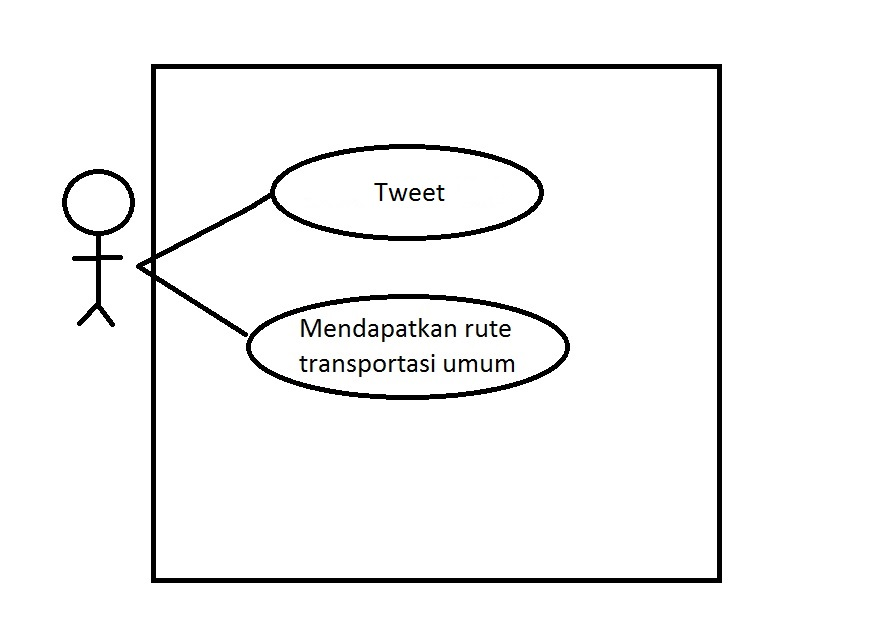
\includegraphics{Gambar/usecase.jpg}
	\caption{Use case Twitter Bot}
	\label{fig:usecase}
\end{figure}

\paragraph{Skenario \textit{Use Case}}
Skenario ini hanya memiliki satu aktor yaitu pengguna. \textit{Tweet} mencari informasi transportasi publik pada skenario ini dilakukan dengan melakukan \textit{tweet} kepada akun \textit{Twitter bot} @kviniink berisi format yang sesuai untuk pencarian rute transportasi. 

\begin{table}[h]
	\begin{tabular}{|l|l|}
	\hline
	Nama           & \textit{Tweet} mencari informasi transportasi publik      											                                                                                                              \\ \hline
	Aktor          & Pengguna                                                                                                                       \\ \hline
	Deskripsi      & \begin{tabular}[c]{@{}l@{}}Melakukan \textit{Tweet}\\ (\textit{Tweet} berupa lokasi asal dan lokasi tujuan)\end{tabular}                         \\ \hline
	Kondisi Awal   & Belum menuliskan \textit{Tweet} pada kolom update                                                                                       \\ \hline
	Kondisi Akhir  & Sudah melakukan \textit{Tweet} kepada user @kiriupdate                                                                                  \\ \hline
	Skenario Utama & \begin{tabular}[c]{@{}l@{}}Pengguna melakukan \textit{Tweet} kepada \textit{user}\\ @kiriupdate dengan format yang sudah ditentukan\end{tabular} \\ \hline
	Eksepsi        & Format penulisan salah                                                                                                         \\ \hline
	\end{tabular}
	\caption{Skenario \textit{Tweet} mencari informasi transportasi }
	\label{tab:SkenarioTweetMencariInformasiTransportasi}
\end{table}

\subsection{\textit{Class Diagram}}
Untuk membuat \textit{class diagram Twitter bot} untuk mencari jalur transportasi publik, dibutuhkan kebutuhan kelas dari skenario. Pada tabel skenario ~\ref{tab:SkenarioTweetMencariInformasiTransportasi}, masukan akan terjadi hal-hal seperti dibawah ini:
\begin{enumerate}
	\item \textit{Twitter bot} akan berjalan terus hingga \textit{Twitter bot} di non-aktifkan.
	\item Pengguna melakukan \textit{tweet} mencari informasi transportasi dengan cara melakukan \textit{mention} kepada akun \textit{Twitter bot} @kviniink dengan format yang sesuai dengan ketentuan.
	\item \textit{Twitter bot} menerima \textit{mention} dari pengguna.
	\item \textit{Twitter bot} akan mencari jalur transportasi publik.
	\item \textit{Twitter bot} melalukan \textit{reply} kepada pengguna yang berisi jalur transportasi publik yang harus ditempuh. 
\end{enumerate}

Berikut adalah \textit{class diagram} sederhana:
\begin{figure}[htbp]
	\centering
		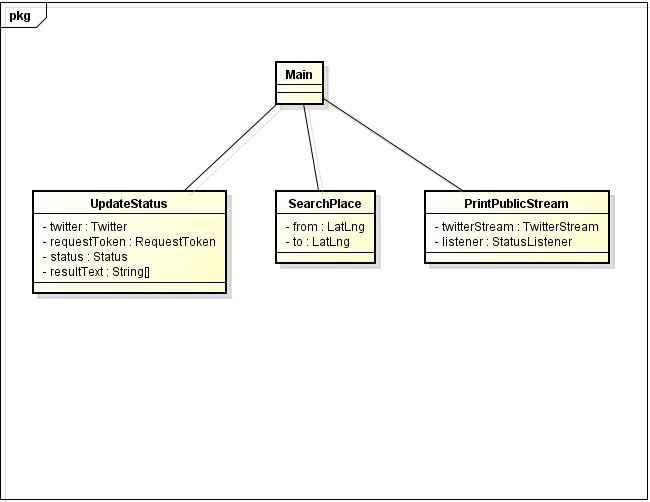
\includegraphics{Gambar/diagramClass.jpg}
	\caption{\textit{Class Diagram} Twitter Bot}
	\label{fig:classdiagram}
\end{figure}